\section{Model Description} \label{sec:model}

%% Contents
% Description of benchmark
% Timestepping, mesh, group constants
% Coupling details for each Step where applicable

\subsection{CNRS multiphysics benchmark}

The \textit{CNRS benchmark} \citep{tiberga_results_2020} is a numerical
benchmark for multiphysics software dedicated to modeling \glspl{MSR}. It
consists of three \textit{phases} and eight \textit{steps} in total. Each
\textit{step} is a well-defined subproblem for systematically assessing the
capabilities of \gls{MSR} software and pinpointing sources of discrepancies
between software. \textit{Phase 0} consists single-physics problems in fluid
dynamics, neutronics, and temperature, respectively. \textit{Phase 1} consists
of coupled, steady-state problems. Lastly, \textit{Phase 2} consists of a
coupled, time-dependent problem.

\begin{figure}[htb!]
	\begin{center}
		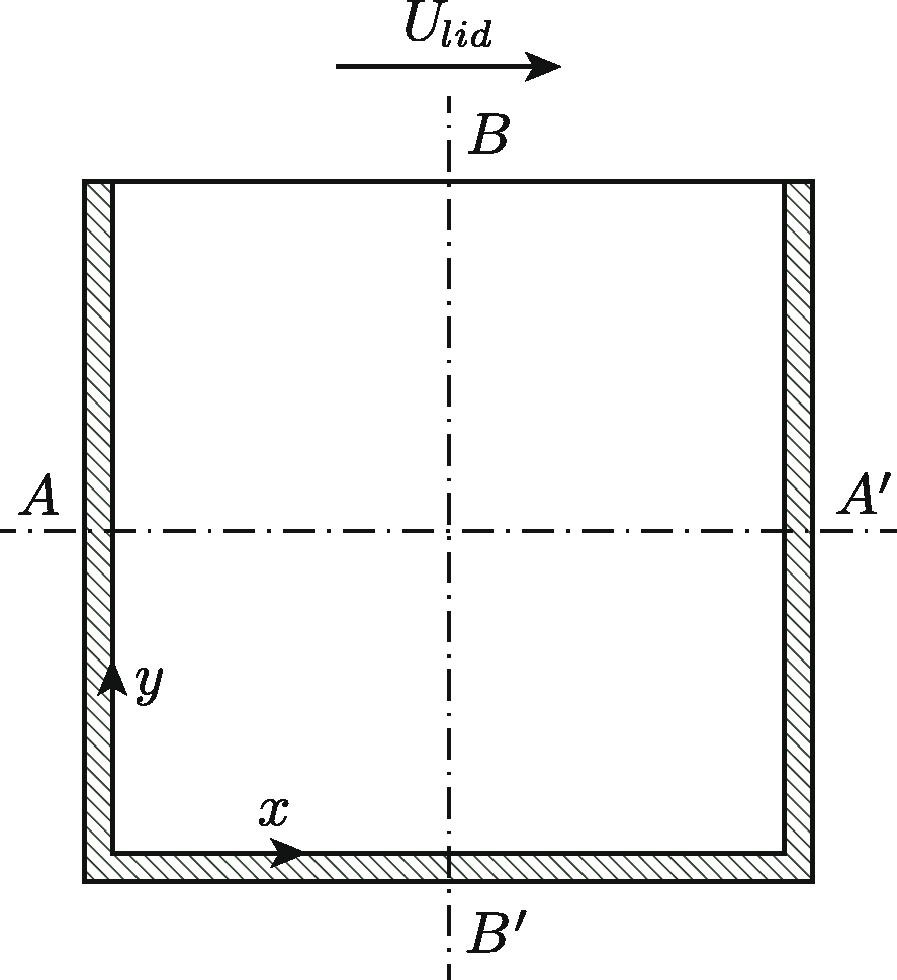
\includegraphics[width=.8\columnwidth]{geometry}
	\end{center}
	\caption{2 m by 2 m domain of the \textit{CNRS benchmark}. $U_{lid}$
	represents the velocity along the top boundary. Various quantities are
	measured along the centerlines AA' and BB' for comparison. From
	\cite{tiberga_results_2020}.}
	\label{fig:geometry}
\end{figure}

As shown in Figure \ref{fig:geometry}, the domain geometry is a 2m by 2m square
cavity filled with LiF-BeF$_2$-UF$_4$ molten salt at an initial temperature of
900K \citep{tiberga_results_2020}.
Standard vacuum boundary conditions apply for neutron flux along all
boundaries, whereby outgoing neutrons are considered lost, while homogeneous
boundary conditions apply for delayed neutron precursors. No-slip boundary
conditions apply for velocity variables in the cavity, except along the top
boundary when the subproblem imposes forced flow in the form of lid-driven
cavity flow. For the temperature variable, all boundaries are insulated and we
simulate salt cooling with the following volumetric heat sink equation:
%
\begin{align}
    q'''(\vec{r}) &= \gamma \left(900 - T(\vec{r})\right), \label{eq:heat}
    \intertext{where}
    q''' &= \mbox{volumetric heat sink [W$\cdot$m$^{-3}$],}
    \nonumber \\
    \gamma &= \mbox{heat transfer coefficient [W$\cdot$m$^{-3}\cdot$K$^{-1}$],}
    \nonumber \\
    T(\vec{r}) &= \mbox{temperature at point $(\vec{r})$ [K].} \nonumber
\end{align}

\cite{tiberga_results_2020} used Serpent 2
\citep{leppanen_serpent_2014} with the JEFF-3.1 library
\citep{koning_jeff-31_2006} to generate multigroup neutronics data for the
LiF-BeF$_2$-UF$_4$ salt in the domain at 900K, condensed into six energy groups
and eight precursor groups. We direct readers to their paper for the
group constant data \citep{tiberga_results_2020}. In addition, the benchmark
prescribes the following equations to govern the temperature dependence in the
cross sections and the neutron diffusion coefficients:
%
\begin{align}
    \Sigma_i (T) &= \Sigma_i(T_{ref})
    \frac{\rho_{fuel}(T)}{\rho_{fuel}(T_{ref})}, \\
    D (T) &= D(T_{ref})
    \frac{\rho_{fuel}(T_{ref})}{\rho_{fuel}(T)},
    \intertext{where}
    \Sigma_i &= \mbox{relevant macroscopic cross section [cm${-1}$],}
    \nonumber \\
    D &= \mbox{neutron diffusion coefficient [cm$^2\cdot$s$^{-1}$],}   
    \nonumber \\
    \rho_{fuel} &= \mbox{density of the fuel salt [kg$\cdot$m$^{-3}$],}
    \nonumber \\
    T_{ref} &= \mbox{reference temperature} = 900\mbox{ K}. \nonumber
\end{align}

The benchmark also prescribes for incompressible Navier-Stokes flow and the
Boussinesq approximation for buoyancy when evaluating the salt flow in the
domain, but places no restrictions on the type of neutronics model.
Table \ref{table:benchmark} briefly details each benchmark subproblem.

\begin{table*}[p!]
	\caption{Description of each benchmark subproblem.}
	\centering
	\small
	\setlength\tabcolsep{2.2pt}
	\begin{tabular}{p{33mm} p{65mm} l p{40mm}<{\centering}}
		\toprule
		Step & Description & Input parameters & Observables \\
		\midrule
		Step 0.1: Velocity field & Solve for the steady-state incompressible
		flow solution from lid-driven cavity flow. &
		$\begin{aligned}[t]
		    U_{lid} &= 0.5 \mbox{ m$\cdot$s$^{-1}$}
        \end{aligned}$
        & $(u_x, u_y)$ along AA' and BB'; \\
        \midrule
        Step 0.2: Neutronics & Solve for the fission rate density
        $\sum^G_i \Sigma_{f,i} \phi_i(\vec{r})$ and reactivity $\rho$
        in a static, isothermal fuel configuration. &
		$\begin{aligned}[t]
		    U_{lid} &= 0 \mbox{ m$\cdot$s$^{-1}$} \\
		    T &= 900 \mbox{ K} \\
		    P &= 1 \mbox{ GW}
        \end{aligned}$
        & $\sum^G_i \Sigma_{f,i} \phi_i(\vec{r})$ along AA'; \newline
        $\rho$; \\
        \midrule
        Step 0.3: Temperature & Solve for the temperature distribution $T$
        arising from the velocity field $(u_x, u_y)_{s_{0.1}}$ and fission heat
        generation $Q_{s_{0.2}}$ from Steps
        0.1 and 0.2, respectively, and a volumetric heat sink (Equation
        \ref{eq:heat}). &
		$\begin{aligned}[t]
		    (u_x, u_y) &= (u_x, u_y)_{s_{0.1}} \\
		    Q &= Q_{s_{0.2}} \\
		    \gamma &= 10^6 \mbox{ W$\cdot$m$^{-3}\cdot$K$^{-1}$}
        \end{aligned}$
        & $T$ along AA' and BB'; \\
        \midrule
        Step 1.1: Circulating fuel & Solve for the delayed neutron source
        distribution $\sum_j \lambda_j C_j$ and reactivity $\rho$ in a
        non-static, isothermal fuel configuration. &
		$\begin{aligned}[t]
		    (u_x, u_y) &= (u_x, u_y)_{s_{0.1}} \\
		    T &= 900 \mbox{ K} \\
		    P &= 1 \mbox{ GW}
        \end{aligned}$
        & $\sum_j \lambda_j C_j$ along AA' and BB'; \newline $\rho -
        \rho_{s_{0.2}}$; \\
        \midrule
        Step 1.2: Power coupling & Solve for the temperature distribution $T$,
        reactivity $\rho$, and fission rate density
        $\sum^G_i \Sigma_{f,i} \phi_i(\vec{r})$ under the fixed velocity field
        from Step 0.1. &
		$\begin{aligned}[t]
		    (u_x, u_y) &= (u_x, u_y)_{s_{0.1}} \\
		    P &= 1 \mbox{ GW} \\
		    \gamma &= 10^6 \mbox{ W$\cdot$m$^{-3}\cdot$K$^{-1}$}
        \end{aligned}$
        & $T$ along AA' and BB'; \newline $\rho - \rho_{s_{1.1}}$; \newline
        $\sum^G_i \Sigma_{f,i} \phi_i(\vec{r}) -
        \left[\sum^G_i \Sigma_{f,i} \phi_i(\vec{r})\right]_{s_{0.2}}$; \\
        \midrule
        Step 1.3: Buoyancy & Solve for the velocity components $(u_x, u_y)$,
        temperature distribution $T$, delayed neutron source
        distribution $\sum_j \lambda_j C_j$, and
        reactivity $\rho$ in a fully coupled system. &
		$\begin{aligned}[t]
		    P &= 1 \mbox{ GW} \\
		    U_{lid} &= 0 \mbox{ m$\cdot$s$^{-1}$} \\
		    \gamma &= 10^6 \mbox{ W$\cdot$m$^{-3}\cdot$K$^{-1}$}
        \end{aligned}$
        & $(u_x, u_y)$ along AA' and BB'; \newline $T$ along AA' and BB';
        \newline $\sum_j \lambda_j C_j$ along AA' and BB'; \newline
        $\rho - \rho_{s_{0.2}}$; \\
        \midrule
        Step 1.4: Full coupling & Solve for the
        reactivity $\rho$ in a fully coupled system with both external
        momemtum-driven flow and buoyancy effects and various permutations of
        $P$ and $U_{lid}$ values.  &
		$\begin{aligned}[t]
		    \gamma &= 10^6 \mbox{ W$\cdot$m$^{-3}\cdot$K$^{-1}$} \\
		    P &= [0, 1] \mbox{ GW} \\
		    U_{lid} &= [0, 0.5] \mbox{ m$\cdot$s$^{-1}$}
        \end{aligned}$
        & $\rho - \rho_{s_{0.2}}$; \\
        \midrule
        Step 2.1: Forced convection transient & Solve* for the
        power gain and phase shift (Bode diagrams) in response to a uniform
        perturbation in the volumetric heat transfer $\gamma$ according to a
        sine wave of amplitude 10\% and frequency $f \in [0.0125, 0.025, 0.05,
        0.1, 0.2, 0.4, 0.8]$ Hz &
		$\begin{aligned}[t]
		    \gamma &= 10^6 \mbox{ W$\cdot$m$^{-3}\cdot$K$^{-1}$} \\
		    P &= [0, 1] \mbox{ GW} \\
		    U_{lid} &= [0, 0.5] \mbox{ m$\cdot$s$^{-1}$}
        \end{aligned}$ &
        $\begin{aligned}
            \text{gain} =& \frac{\left(P_{max} - P_{avg}\right)/P_{avg}}{
            \left(\gamma_{max} - \gamma_{avg}\right)/\gamma_{avg}}; \\
            \text{phase}& \text{ shift} = \theta_P - \theta_\gamma;
        \end{aligned}$ \\
		\bottomrule
	\end{tabular}
	\label{table:benchmark}
\end{table*}

\subsection{Modeling approach}

% Timestepping, mesh, group constants
% Coupling details for each Step where applicable

For this work, we ran the benchmark cases on a uniformly-spaced mesh consisting
of 200 by 200 elements. Thus, the dimensions of each mesh element are 0.01m by
0.01m. We
approximated most of the relevant variables, i.e. neutron fluxes, velocity
components, pressure, and temperature, using first-order Lagrange shape
functions. The only exception is the precursor concentration variables, which
we approximated using zeroth-order monomial shape functions and solved using
\gls{DFEM}. We took the group constant data directly from
\cite{tiberga_results_2020} and rewrote it into the Moltres-compatible text
format without any other modifications.

As mentioned in Section \ref{sec:moltres}, \gls{MOOSE}'s \textit{Navier-Stokes}
and \textit{Heat Conduction} modules provide some of the capabilities for
modeling incompressible flow and heat transfer. In particular, we stabilized
the incompressible flow and temperature governing equations using the
streamline upwind Petrov-Galerkin and pressure-stabilizing Petrov-Galerkin
stabilization methods \citep{peterson_overview_2017} implemented in
\gls{MOOSE}. Without these stabilization techniques, we observed spurious
numerical oscillations in the velocity and temperature. These oscillations are
commonly reported when using finite element methods to solve
advection-dominated flow and lid-driven cavity problems with corner
singularities where different boundary conditions meet
\citep{kuhlmann_lid-driven_2018}.

We performed all simulations using the Preconditioned \gls{JFNK} solver from
the \gls{MOOSE} framework. The coupled steady-state problems in
\textit{Steps 1.3} and \textit{1.4} required loose coupling between neutronics
and thermal-hydraulics due to the unique problem setup involving an eigenvalue
problem for the neutron multiplication factor and a standard steady-state
problem in thermal-hydraulics simultaneously. All other multiphysics problems
in \textit{Steps} in \textit{Phases 1} and \textit{2} were fully coupled
within the same \gls{JFNK} solve.

For the time-dependent cases in \textit{Step 2.1}, we used a second-order
implicit Backward Differential Formula (BDF2) time-stepping scheme and fixed
the timestep sizes at 1/200 of the period of the corresponding driving
frequencies as shown in Table \ref{table:timestep}. The only exception is the
0.8 Hz case as a timestep size of 0.4s required more than one hundred nonlinear
iterations to converge in each timestep.

\begin{table}[htb!]
    \caption{Timestep sizes used for the time-dependent cases in
    \textit{Step 2}.}
	\centering
	\setlength\tabcolsep{2.5pt}
	\begin{tabular}{l S S S S S S S}
	    \toprule
	    Frequency [Hz] & 0.0125 & 0.025 & 0.05 & 0.1 & 0.2 & 0.4 & 0.8 \\
	    \midrule
	    Timestep size [s] & 0.2 & 0.2 & 0.1 & 0.05 & 0.025 & 0.0125 & 0.00625
	    \\
	    \bottomrule
	\end{tabular}
	\label{table:timestep}
\end{table}
